%%%%%%%%%%%%%%%%%%%%%%%%%%%%%%%%%%%%%%%%%
% Programming/Coding Assignment
% LaTeX Template
%
% This template has been downloaded from:
% http://www.latextemplates.com
%
% Original author:
% Ted Pavlic (http://www.tedpavlic.com)
%
% Note:
% The \lipsum[#] commands throughout this template generate dummy text
% to fill the template out. These commands should all be removed when 
% writing assignment content.
%
% This template uses a Perl script as an example snippet of code, most other
% languages are also usable. Configure them in the "CODE INCLUSION 
% CONFIGURATION" section.
%
%%%%%%%%%%%%%%%%%%%%%%%%%%%%%%%%%%%%%%%%%

%----------------------------------------------------------------------------------------
%	PACKAGES AND OTHER DOCUMENT CONFIGURATIONS
%----------------------------------------------------------------------------------------

\documentclass{article}
\usepackage{fullpage}
\usepackage[numbers]{natbib}
\usepackage{url}
\usepackage{float}
\usepackage{hyperref}
\usepackage{fancyhdr} % Required for custom headers
\usepackage{lastpage} % Required to determine the last page for the footer
\usepackage{extramarks} % Required for headers and footers
\usepackage[usenames,dvipsnames]{color} % Required for custom colors
\usepackage{graphicx} % Required to insert images
\usepackage{listings} % Required for insertion of code
\usepackage{courier} % Required for the courier font
\usepackage{lipsum} % Used for inserting dummy 'Lorem ipsum' text into the template
\usepackage{color}
\usepackage{enumerate}
\usepackage{algpseudocode}
\usepackage{algorithm}
\usepackage{mips}
\usepackage{siunitx} % Provides the \SI{}{} and \si{} command for typesetting SI units
\usepackage{amsmath} % Required for some math elements 
\usepackage{natbib} % Required to change bibliography style to APA
\usepackage{cases}
\usepackage{mathtools}
\lstloadlanguages{C}


\definecolor{dkgreen}{rgb}{0,0.6,0}
\definecolor{gray}{rgb}{0.5,0.5,0.5}
\definecolor{mauve}{rgb}{0.58,0,0.82}
\lstset{ %
  language=[mips]Assembler,       % the language of the code
  basicstyle=\footnotesize,       % the size of the fonts that are used for the code
  numbers=left,                   % where to put the line-numbers
  numberstyle=\tiny\color{gray},  % the style that is used for the line-numbers
  stepnumber=1,                   % the step between two line-numbers. If it's 1, each line 
                                  % will be numbered
  numbersep=5pt,                  % how far the line-numbers are from the code
  backgroundcolor=\color{white},  % choose the background color. You must add \usepackage{color}
  showspaces=false,               % show spaces adding particular underscores
  showstringspaces=false,         % underline spaces within strings
  showtabs=false,                 % show tabs within strings adding particular underscores
  frame=single,                   % adds a frame around the code
  rulecolor=\color{black},        % if not set, the frame-color may be changed on line-breaks within not-black text (e.g. commens (green here))
  tabsize=4,                      % sets default tabsize to 2 spaces
  captionpos=b,                   % sets the caption-position to bottom
  breaklines=true,                % sets automatic line breaking
  breakatwhitespace=false,        % sets if automatic breaks should only happen at whitespace
  title=\lstname,                 % show the filename of files included with \lstinputlisting;
                                  % also try caption instead of title
  keywordstyle=\color{blue},          % keyword style
  commentstyle=\color{dkgreen},       % comment style
  stringstyle=\color{mauve},         % string literal style
  escapeinside={\%*}{*)},            % if you want to add a comment within your code
  morekeywords={*,...}               % if you want to add more keywords to the set
}

\setlength\parindent{0pt} % Removes all indentation from paragraphs

\renewcommand{\labelenumi}{\alph{enumi}.} % Make numbering in the enumerate environment by letter rather than number (e.g. section 6)

%\usepackage{times} % Uncomment to use the Times New Roman font

%----------------------------------------------------------------------------------------
%	DOCUMENT INFORMATION
%----------------------------------------------------------------------------------------

\title{EE3450 Project \#1: MIPS Assembly Programming} % Title

\author{Chi-Ming Lee} % Author name
\date{\today} % Date for the report

\begin{document}

\maketitle % Insert the title, author and date

\begin{center}
\begin{tabular}{l r}
    Instructor: Yarsun Hsu
\end{tabular}
\end{center}

\begin{center}
\begin{tabular}{l r}
Due date: November 29, 2015 % Instructor/supervisor
\end{tabular}
\end{center}

% If you wish to include an abstract, uncomment the lines below
% \begin{abstract}
% Abstract text
% \end{abstract}

%----------------------------------------------------------------------------------------
%	SECTION 1
%----------------------------------------------------------------------------------------

\section{Objective}

In this project, you will implement several classical algorithms that determine the Fibonacci number\cite{fibref} with MIPS assembly. 
In addition to coding, we will use MARS\cite{marsref} as the simulation tool to perform analysis and comparison on these algorithms.
The definition of Fibonacci number is shown below:

\begin{equation*}
    F_{n} = 
    \begin{cases}
        0 & (n = 0)\\
        1 & (n = 1)\\
        F_{n-1}+F_{n-2} & (n > 1)
    \end{cases}
\end{equation*}


We will enumerate five algorithms for you. For each of them, please do the following:
\begin{enumerate}
    \item Use the described method to solve the Fibonacci number with C.
    \item Use the described method to solve the Fibonacci number with MIPS assembly and verify your result with the C version.
    \item Organize statistics from MARS and use your favorite tool (Excel, Matlab, gnuplot, etc.) to \textbf{plot a graph} that illustrates relationship between input size and total instruction count. 
\end{enumerate}
All your programs need to be explained explicitly and carefully with \textbf{comments in source codes} because they are the important part of grading.
\textbf{Do not copy your codes into the report} but instead discuss your insight into algorithms or the key idea of your implementation.\\

After you are done with these algorithms and plots, you must perform analysis and comparison on them with various metrics in your report. For examples:
\begin{itemize}
    \item Complexity
    \item Code size
    \item Instruction type distribution
\end{itemize}
You might further discuss how an algorithm trade off among these (or more) metrics, what is the distribution of instruction types in an algorithm (this affects instruction per cycle), and so on. 
There is no standard template for this report, but you need to \textbf{make a conclusion} (e.g., what you have learned or accomplished) in the end of it.
Note that \textbf{coding (including comments) and the report will take identical proportion} in this project.

%----------------------------------------------------------------------------------------
%	SECTION 2
%----------------------------------------------------------------------------------------
\section{Problem Statements}

\subsection{Problem A: Iterative Method}
The iterative method begins with the determined part of the problem (i.e. $F_{0}$ and $F_{1}$), and approaches the final result step by step as follows:

\begin{align*}
    \begin{aligned}
        F_{0} &= 0, F_{1} = 1 \\
    \rightarrow F_{2} &= F_{1} + F_{0} = 1 + 0 = 1\\
    \rightarrow F_{3} &= F_{2} + F_{1} = 1 + 1 = 2\\
    \rightarrow F_{4} &= F_{3} + F_{2} = 2 + 1 = 3\\
    ....
    \end{aligned}
\end{align*}

You will need a loop to implement such iterations in your program. To illustrate this method more concretely, let's take an example from another problem, Factorial number, which is defined below:
%For your reference, we provide sample codes that use 
%iterative method to solve another problem, Factorial number, which is defined below:
\begin{equation*}
    n! = 
    \begin{cases}
        1 & (n = 0)\\
        \prod^{n}_{k=1}k & (n > 0)
    \end{cases}
\end{equation*}

The iterative-method sample codes solving Factorial are shown below:
\lstinputlisting[language=C]{fac_ite.c}
\lstinputlisting{fac_ite.asm}
You might reference the samples to implement your Fibonacci programs.

%----------------------------------------------------------------------------------------
%	SECTION 3
%----------------------------------------------------------------------------------------

\subsection{Problem B: Recursive Method}

The recursive method\cite{recref} solves the problem by partitioning it into sub-problems level by level, and then combines sub-solutions into the final result.
Procedure call in programming language provides us an intuitive way to implement such a recursive method. 
The programmer can partition the problem by calling the same procedure with smaller input, and then combine values into the final solution. Please make sure you are familiar with MIPS calling convention \cite{callref} before doing this problem.
Again, we take factorial number as an example with its recursive form:

\begin{equation*}
    n! = 
    \begin{cases}
        1 & (n = 0)\\
        n\times(n-1)! & (n > 0)
    \end{cases}
\end{equation*}


Sample codes are shown below:
\lstinputlisting[language=C]{fac_rec.c}
\lstinputlisting{fac_rec.asm}
You might reference the samples to implement your Fibonacci programs.

%----------------------------------------------------------------------------------------
%	SECTION 4
%----------------------------------------------------------------------------------------

\subsection{Problem C: Tail Recursion}

    Suppose you have completed problem B, you might notice its instruction count grows greatly with input size. To address this issue, some programmers might use "tail recursion" to improves the efficiency of the original recursion. Please reference \cite{tailref} and discuss how the tail recursion out-performs the original one in Problem B. The pseudo code of tail recursion that solves Fibonacci number is shown in the Algorithm 1.

\renewcommand{\algorithmicrequire}{\textbf{Input:}}
\renewcommand{\algorithmicensure}{\textbf{Output:}}

\begin{algorithm}[H]
    \caption{Tail Recursion Solving Fibonacci}
\begin{algorithmic}
    \Require{$n$}(Integer)
    \Ensure{$F_{n}$}(Integer) \\
    \State $F_{n} \gets $ \Call{Tail\_Recursion}{$n-1$, $0$, $1$} 
    \State \Return $F_{n}$ \\

    \Function{Tail\_Recursion}{$k$, $a$, $b$}
        \If {$k == 0$} \Return $a$
        \Else \Call {Tail\_Recursion}{$k-1$, $b$, $a+b$}
        \EndIf
    \EndFunction
\end{algorithmic}
\end{algorithm}


%----------------------------------------------------------------------------------------
%	SECTION 5
%----------------------------------------------------------------------------------------

\subsection{Problem D: Q Matrix}

The Q matrix method\cite{qmat} accelerates finding Fibonacci number by manipulating matrix multiplication shown below:

\begin{align}
    \begin{bmatrix} F_{n+1}&F_{n} \\ F_{n}&F_{n-1} \end{bmatrix} 
                           &= \begin{bmatrix} F_{n} + F_{n-1}& F_{n-1} + F_{n-2} \\ F_{n-1}+F_{n-2}&F_{n-2}+F_{n-3} \end{bmatrix} \\
                           &= \begin{bmatrix} 1&1 \\ 1&0 \end{bmatrix} \times \begin{bmatrix} F_{n}&F_{n-1} \\ F_{n-1}&F_{n-2} \end{bmatrix} \\
    \shortintertext{Repeat above k times, (1) becomes:}
                           &\rightarrow  \begin{bmatrix} 1&1 \\ 1&0 \end{bmatrix}^{k} \times \begin{bmatrix} F_{(n+1)-k}&F_{n-k} \\ F_{n-k}&F_{(n-1)-k} \end{bmatrix}
    \shortintertext{In (3) let:}
\begin{bmatrix} 1&1 \\ 1&0 \end{bmatrix} &=Q\\
                         k &= n-1
    \shortintertext{We have:}
    \begin{bmatrix} F_{n+1}&F_{n} \\ F_{n}&F_{n-1} \end{bmatrix} 
                           &= Q^{n-1} \times \begin{bmatrix} F_{2}&F_{1} \\ F_{1}&F_{0} \end{bmatrix} \\
                           &= Q^{n-1} \times \begin{bmatrix} 1 & 1 \\ 1&0 \end{bmatrix} \\
                           &= Q^{n}
\end{align}
 
By this formula, we can get $F_{n}$ directly by finding $Q^{n}$. Nevertheless, multiplying with $Q$ n times is not an efficient approach.
Instead, the Q matrix algorithm solves $Q^{n}$ by finding square root of it recursively. Let's take an example of $n = 16$
\begin{equation*}
    Q^{16} = Q^{8}Q^{8} = (Q^{4}Q^{4}) (Q^{4}Q^{4}) = ...
\end{equation*}
However, the power of $Q$ will be an odd number very likely. In such a scenario, you will need some trivial work to partition it carefully. Let's take another example of $n = 5$
\begin{equation*}
    Q^{5} = Q^{3}Q^{2} = (Q^{2}Q^{1}) (Q^{1}Q^{1}) = [(Q^{1}Q^{1}) Q^{1}] (Q^{1}Q^{1})
\end{equation*}

The pseudo code of this method is organized in Algorithm 2.

\begin{algorithm}[H]
\caption{Q Matrix Solving Fibonacci}

\begin{algorithmic}
    \Require{$n$ (Integer), $Q^1$ (Matrix)}
    \Ensure{$F_{n}$ (Integer)} \\

    \State  $Q^{n} \gets$ \Call {Find\_Q\_Matrix}{$n$}
    \State $F_{n} \gets Q^{n}[0][1]$ 
    \State \Return $F_{n}$\\

    \Function{Find\_Q\_Matrix}{$k$}
    \If{$k==1$}
        \Return $Q^1$
    \ElsIf{$k \in \text{Even number}$ }
        \State $Q^{\frac{k}{2}} \gets$ \Call {Find\_Q\_Matrix}{$\frac{k}{2}$}
        \Return $Q^{\frac{k}{2}} \times Q^{\frac{k}{2}}$
    \ElsIf{$k \in \text{Odd number}$ }
        \State $Q^{\frac{k}{2}} \gets$ \Call {Find\_Q\_Matrix}{$\frac{k}{2}$}
        \State $Q^{\frac{k}{2}+1} \gets$ \Call {Find\_Q\_Matrix}{$\frac{k}{2} + 1$}
        \Return $Q^{\frac{k}{2}} \times Q^{\frac{k}{2}+1}$
    \EndIf
        
    \EndFunction


\end{algorithmic}
\end{algorithm}

Here are two hints for this problems:
\begin{enumerate}
    \item We usually need 3 level loops to implement matrix multiplication \cite{matrix}. 
        In this case, however, unrolling loops (i.e., writing all addition and multiplication manually instead using loops) might make this problem easier because only 2 by 2 matrices are involved.
    \item Before doing matrix multiplication, we must allocate memory for the result matrix. 
        This can be done by the function "malloc"\cite{malloc} in C and "syscall 9"\cite{syscall9} in MIPS.
\end{enumerate}

Provided template C and MIPS codes with mmul (matrix multiplication) functions that can be used directly might be helpful in this problem, but \textbf{they are not golden implementation.} You might improve it too get bonus.
\lstinputlisting[language=C]{fib_template.c}
\lstinputlisting{fib_template.asm}


%----------------------------------------------------------------------------------------
%	SECTION 6
%----------------------------------------------------------------------------------------

\subsection{Problem E: Fast Doubling Method}
The fast doubling\cite{fast} method uses a bottom-up approach to solve $A^n$ rather than a top-down one used in the Q matrix method.
The idea of fast doubling comes from Q matrix:


\begin{align}
    \shortintertext{Let:}
    \begin{bmatrix} F_{2n+1} \\ F_{2n}\end{bmatrix} &= \begin{bmatrix} F_{2n+1}&F_{2n} \\ F_{2n}&F_{2n-1} \end{bmatrix} \begin{bmatrix} 1 \\ 0 \end{bmatrix} \\
    \shortintertext{Use the equation of Q matrix:}
    \begin{bmatrix} F_{n+1}&F_{n}\\F_{n}&F_{n-1}\end{bmatrix} &= \begin{bmatrix} 1&1 \\ 1&0 \end{bmatrix}^{n}
    \shortintertext{(9) can be written as:}
                                        \begin{bmatrix} 1&1 \\ 1&0 \end{bmatrix}^{2n} \begin{bmatrix} 1 \\ 0 \end{bmatrix} 
                                        &= \begin{bmatrix} 1&1 \\ 1&0 \end{bmatrix}^{n}  \begin{bmatrix} 1&1 \\ 1&0 \end{bmatrix}^{n} \begin{bmatrix} 1 \\ 0 \end{bmatrix} \\
                                        &= \begin{bmatrix} F_{n+1}&F_{n}\\F_{n}&F_{n-1}\end{bmatrix} \begin{bmatrix} F_{n+1}&F_{n}\\F_{n}&F_{n-1}\end{bmatrix} \begin{bmatrix} 1 \\ 0 \end{bmatrix} \\
                                        &= \begin{bmatrix} F_{n+1}^2+F_{n}^2 \\ F_{n}(F_{n+1}+F_{n-1})\end{bmatrix}
    \shortintertext{In (13) let:}
                                 F_{n-1}&= F_{n+1} - F_{n}
    \shortintertext{We get the fast doubling formula:}
                                           F_{2n+1}   &= F_{n+1}^2 + F_{n}^2 \\
                                           F_{2n} &= F_{n}(2F_{n+1}-F_{n}) 
\end{align}

With this formula, we can find $F_{2n+1}$ and $F_{2n}$ simply by manipulating $F_{n+1}$ and $F_{n}$. 
The figure below illustrates how the fast doubling works: \\
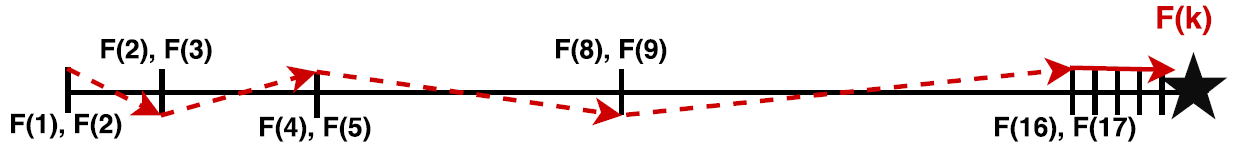
\includegraphics[width=\textwidth]{fast}
The fast doubling begins with $F_{1} = 1$ and $F_{2} = 1$, and doubles its index iteration by iteration.
As soon as the index closes enough with the target, the algorithm switches to the iterative method and gets the final result.

The pseudo code is organized in the Algorithm 3.
 
\begin{algorithm}
\caption{Fast Doubling Solving Fibonacci}
\begin{algorithmic}
    \Require $n$ (Integer)
    \Ensure $F_{n}$ (Integer)
    \If{$n==0$} \Return {$0$} 
    \EndIf
        \State $i \gets 1$; $F_{i} \gets 1$; $F_{i+1} \gets 1$
    \While { $i < n$}
    \If{$i \leq \frac{n}{2}$}
        \State $F_{2i+1} \gets F_{i}^2 + F_{i+1}^2$; $F_{2i} \gets F_{i} \times (2F_{i+1} - F_{i})$
        \State $F_{i} \gets F_{2i}$; $F_{i+1} \gets F_{2i+1}$
        \State $i \gets i \times 2$
    \Else
        \State $F_{i+2} \gets F_{i+1} + F_{i}$ 
        \State $F_{i} \gets F_{i+1}$
        \State $F_{i+1} \gets F_{i+2}$
        \State $i \gets i+1$
    \EndIf
    \EndWhile 
    \State \Return $F_{i+1}$
\end{algorithmic}
\end{algorithm}


\section{What to submit}
\textbf{This is the most important section. Your codes might fail if you ignore anything in this section.}
\begin{itemize}
    \item Five C codes, fibA.c, fibB.c, fibC.c, fibD.c and fibE.c, described as section 2\\
        You must make sure all your C codes can be tested in the terminal of EE workstation as follows: 
        \begin{enumerate}
            \item In the folder of your C codes
            \item Enter: gcc fibA.c
            \item Enter: ./a.out
            \item Enter: 10
            \item Terminal shows nothing but "55"
        \end{enumerate}
        Please do not print anything else on the terminal.
    \item Five MIPS codes, fibA.asm, fibB.asm, fibC.asm, fibD.asm and fibE.asm, described as section 2\\
        You must make sure all your MIPS codes can be tested in MARS follows: 
        \begin{enumerate}
            \item Load fibA.asm
            \item Run
            \item Enter: 10
            \item The console shows "55" and the system information "-- program is finished running --"
        \end{enumerate}
    \item A PDF report named "ID+report.pdf". For Example, mine is "103061568report.pdf".
\end{itemize}
Please \textbf{zip these 11 items directly without any folder}, and name your zip file as \textbf{"ID+pj1.zip"}. For example, mine is "103061568pj1.zip".

%----------------------------------------------------------------------------------------
%	BIBLIOGRAPHY
%----------------------------------------------------------------------------------------

\bibliographystyle{ieeetr}

\bibliography{pj1}

%----------------------------------------------------------------------------------------


\end{document}
